\documentclass[12pt, aspectratio=141]{beamer}

\definecolor{jrouge}{HTML}{CB3C33}
\definecolor{jvert}{HTML}{389826}
\definecolor{jbleu}{HTML}{4063D8}
\definecolor{jviolet}{HTML}{9558B2}
\definecolor{lightred}{HTML}{fcf3f3}
\definecolor{lightgreen}{HTML}{e1f6db}
\definecolor{lightpurple}{HTML}{f4eef7}
\definecolor{lightgrey}{gray}{0.95}

\mode<presentation>
{
	\usetheme{default}
	\usecolortheme{rose}
	%	\useoutertheme{smoothbars}
	\useinnertheme{circles}
	
	\definecolor{beamer@blendedblue}{HTML}{4063D8}
	%\definecolor{titlemustard}{rgb}{0.6,0.6,0.0}
	%\setbeamercolor{title}{bg=titlemustard}
	\setbeamercolor{normal text}{fg=black}
	\setbeamercolor{alerted text}{fg=jrouge}
	\setbeamerfont{title}{shape=\bfseries}
	\setbeamercolor{example text}{fg=jvert}
	
	%\setbeamercolor{structure}{fg=beamer@blendedblue}
	\setbeamertemplate{navigation symbols}{}
	\setbeamertemplate{footline}{\color{black!50}\hfill\scriptsize\insertpagenumber\hspace{2em}\vspace{2em}}
}

\usepackage{natbib}
%\renewcommand{\citenumfont}[1]{{\tiny#1}}
\renewcommand{\citenumfont}[1]{}
\bibpunct{}{};s;;

\usepackage[french]{babel}
\usepackage[mathletters]{ucs}
\usepackage[utf8x]{inputenc}
\usepackage[T1]{fontenc}
% Or whatever. Note that the encoding and the font should match. If T1
% does not look nice, try deleting the line with the fontenc.
% Alternative for XeLaTeX:
%\usefonttheme{professionalfonts}
%\usepackage{fontspec}
%\setmonofont{JuliaMono}
%\setdefaultlanguage{french}
%\usepackage{unicode-math}

\usepackage{subcaption}

\usepackage{array}
\usepackage{multirow}
\usepackage{setspace}
\usepackage{soul}
\usepackage{amssymb}
\usepackage{mathrsfs}
\usepackage{bbm}
\usepackage{svg}

\usepackage{tikz}
\usetikzlibrary{scopes, backgrounds, arrows, automata, positioning, patterns, calc, decorations.pathmorphing, decorations.pathreplacing, arrows.meta}

\usepackage{hyperref}
\usepackage{ragged2e}
\usepackage{graphicx}
\usepackage{amsmath}
\usepackage{aeguill}

\usepackage{algorithm}
\usepackage{algpseudocode}
\usepackage{stmaryrd}
\usepackage{moresize}

\newcommand{\llbra}{\left\llbracket}
\newcommand{\rrbra}{\right\rrbracket}
\renewcommand{\brack}[1]{\ensuremath{\llbra#1\rrbra}}
\newcommand{\der}[2]{#1^{\ensuremath{\left(#2\right)}}}
\newcommand{\paren}[1]{\ensuremath{\left(#1\right)}}
\newcommand{\abs}[1]{\ensuremath{\left|#1\right|}}
\newcommand{\interval}[1]{\ensuremath{\left[#1\right]}}
\newcommand{\set}[2]{\ensuremath{\left\{#1\,\middle|\,#2\right\}}}
\newcommand{\cont}[1]{\mathcal{C}^{#1}}
\newcommand{\tends}[2]{\underset{#1\to #2}{\longrightarrow}}
\newcommand{\seq}[3]{\ensuremath{\left(#1_{#2}\right)_{#2\in#3}}}
\newcommand{\matr}[2]{\mathcal{M}_{#1}\paren{#2}}
\newcommand{\matrRect}[3]{\mathcal{M}_{#1,#2}\paren{#3}}
\newcommand{\Id}{\text{Id}}
\newenvironment{disj}[1]{\left\{\begin{array}{#1}} {\end{array}\right.}

\usepackage{siunitx}


\newenvironment{changemargin}[2]{%
	\begin{list}{}{%
			%\setlength{\topsep}{0pt}%
			\setlength{\leftmargin}{#1}%
			\setlength{\rightmargin}{#2}%
			\setlength{\listparindent}{\parindent}%
			\setlength{\itemindent}{\parindent}%
			\setlength{\parsep}{\parskip}%
		}%
		\item[]}{\end{list}}

\defbeamertemplate{section page}{mruffel}[1][]{%
	\begin{centering}
		{\usebeamerfont{section name}\usebeamercolor[fg]{section name}#1
			\vskip1em\par
			
			\begin{beamercolorbox}[sep=12pt,center,rounded=true,shadow=true]{part title}
				\usebeamerfont{section title}\insertsection\par
		\end{beamercolorbox}}
	\end{centering}
}



% If you have a file called "university-logo-filename.xxx", where xxx
% is a graphic format that can be processed by latex or pdflatex,
% resp., then you can add a logo as follows:

\pgfdeclareimage[height=0.5cm]{Mines}{../figures/Mines.pdf}
\logo{\begin{tikzpicture}[overlay,remember picture]
		\node[left=0.2cm] at (current page.31){
			\pgfuseimage{Mines}
		};
\end{tikzpicture}}



% Delete this, if you do not want the table of contents to pop up at
% the beginning of each subsection:
%\AtBeginSubsection[]
%{
	%  \begin{frame}<beamer>
		%    \tableofcontents[currentsection,currentsubsection]
		%  \end{frame}
	%}

\AtBeginSection[]
{
	\begin{frame}
		\sectionpage
	\end{frame}
}

% If you wish to uncover everything in a step-wise fashion, uncomment
% the following command: 

%\beamerdefaultoverlayspecification{<+->}

\usepackage{minted}
\usemintedstyle{paraiso-light}
\setminted[julia]{mathescape,linenos,obeytabs,tabsize=4,numbersep=3pt,fontsize=\small,framesep=2mm,autogobble,bgcolor=lightred,escapeinside=££}
\setminted[bash]{mathescape,obeytabs,tabsize=4,numbersep=3pt,fontsize=\small,framesep=2mm,autogobble,bgcolor=lightgrey,escapeinside=££}

\usepackage{lmodern}
%\newcommand{\jl}[1]{\colorbox{lightred}{\small\ttfamily #1}}
\newmintinline[jl]{julia}{}
\newmintinline[jlscript]{julia}{fontsize=\scriptsize}
\newmint[JL]{julia}{}
\newmint[JLa]{julia}{linenos=false}
\newminted{julia}{}
\newenvironment{julia}{\vspace{-0.6em}\VerbatimEnvironment\begin{juliacode}}{\end{juliacode}}
\newminted[jlrepl]{julia}{linenos=false}
\newenvironment{repl}{\vspace{-0.6em}\VerbatimEnvironment\begin{jlrepl}}{\end{jlrepl}}
\newcommand{\q}{\textquotesingle}
\newcommand{\qq}{\textquotedbl}
\newcommand{\jlREPL}{\textcolor{jvert}{\bfseries julia>}}

\DeclareTextFontCommand{\emph}{\color{jrouge}\bfseries}

\newenvironment<>{definition}[1]{%
	\setbeamercolor{block title}{bg=lightgreen}%
	\begin{block}{Définition}{#1}}{\end{block}}

\newenvironment<>{convention}[1]{%
	\setbeamercolor{block title}{bg=lightpurple}%
	\begin{block}{Convention}{#1}}{\end{block}}

\usepackage{xspace}
\newcommand{\expr}{\ensuremath{\left\langle\textit{expr}\right\rangle}\xspace}
\newcommand{\expra}[1]{\ensuremath{\left\langle\textit{expr}_{#1}\right\rangle}\xspace}
\newcommand{\bexpr}{\ensuremath{\left\langle\textit{bexpr}\right\rangle}\xspace}
\newcommand{\bexpra}[1]{\ensuremath{\left\langle\textit{bexpr}_{#1}\right\rangle}\xspace}
\newcommand{\type}{\ensuremath{\left\langle\textit{type}\right\rangle}\xspace}
\newcommand{\typea}[1]{\ensuremath{\left\langle\textit{type}_{#1}\right\rangle}\xspace}


\title{Apprentissage de la programmation en Julia}

\subtitle{Métaprogrammation}

\author{Lionel~Zoubritzky\inst{}}

\institute{Mines Paris -- PSL}

\date{01/2025}

\begin{document}
\setbeamertemplate{section page}[mruffel]

\begin{frame}
	\titlepage
\end{frame}

\begin{frame}[fragile]{Rappels du premier cours}
	\begin{definition}
		Une \emph{expression} est un morceau de code qui a une valeur.
	\end{definition}
	
	Exemple et contre-exemple :
	\begin{itemize}
		\item \jl|3 + 5| : c'est une expression dont la valeur est 8.
		\item \jl|3 +| : ce n'est pas une expression car ce code est incomplet.
	\end{itemize}
	\vfill
	
	\begin{definition}
		Un \emph{littéral} est une expression dont l'écriture donne la valeur.
	\end{definition}
	Exemples : \jl{true}, \jl{-32}, \jl{'ç'}, \jl{"Bonjour !"}, \ldots
\end{frame}

\begin{frame}[fragile]{Arbre de syntaxe abstrait}
	Lorsque le code est lu par le compilateur ou l'interpréteur, il est stocké en mémoire sous une forme organisée qui permet de le transformer jusqu'au code machine. Cette forme est un \emph{arbre de syntaxe abstrait}.
	\vfill
	
	\begin{minipage}{0.38\linewidth}
		Exemple :
		\begin{julia}
			foo(x) = begin
				y = x + 7
				y > 12 && return x
				return y^x
			end
		\end{julia}
	\end{minipage}\hfill%
	\begin{minipage}{0.6\linewidth}
		\centering
		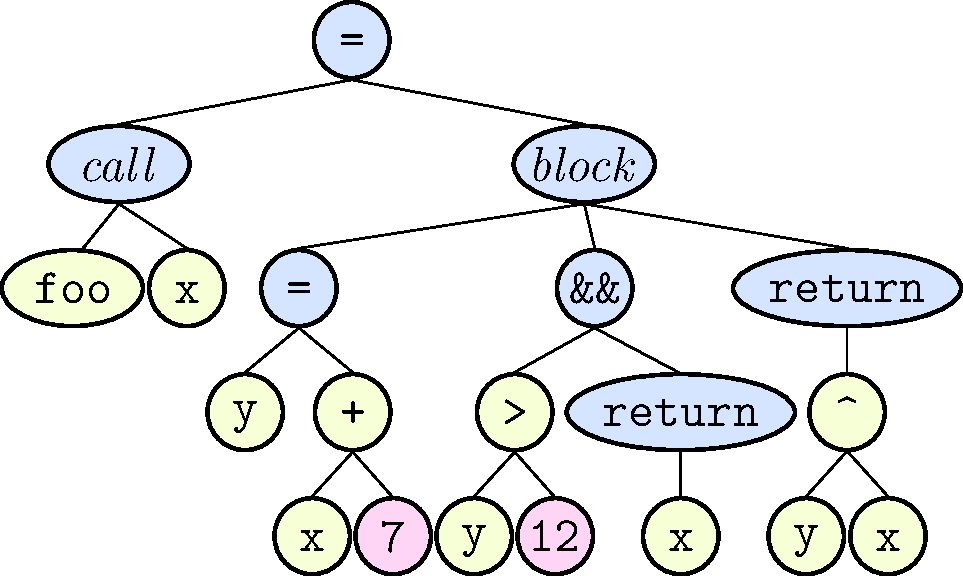
\includegraphics[width=0.9\linewidth]{../figures/ast.pdf}
	\end{minipage}

	\pause\vfill
	En rose les littéraux, en vert les identifiants, en bleu le reste.
\end{frame}

\begin{frame}{Arbre de syntaxe abstrait}
	L'arbre de syntaxe abstrait structure le code en suivant le parenthésage :
	\begin{itemize}
		\item Chaque sous-arbre représente une expression.
		\item Chaque nœud représente une opération élémentaire du langage (affectation, appel de fonction, définition d'un struct, etc.).
		\item Les feuilles sont des expressions dont l'évaluation est immédiate : soit des littéraux, soit des identifiants.
	\end{itemize}

	Un fichier entier de code Julia peut être représenté par un seul arbre ayant pour racine \textit{block}, qui représente un bloc d'instructions à évaluer de gauche à droite.
\end{frame}

\begin{frame}[fragile]{Le type \texttt{Expr}}
	Un arbre de syntaxe abstrait est représentée en Julia par le type \jl{Expr} :
	\begin{julia}
		struct Expr
			head::Symbol
			args::Vector{Any}
		end
	\end{julia}

	Une \expr non évaluée peut être obtenue avec la syntaxe \jl{:(£\expr\!\!\!£)} :
	\begin{repl}
		£\jlREPL£ ex = :(3 + foo(4))
		:(3 + foo(4))
		
		£\jlREPL£ ex.head
		:call
		
		£\jlREPL£ ex.args
		3-element Vector{Any}:
		  :+
		 3
		  :(foo(4))
	\end{repl}
	\vspace{-4em}
\end{frame}

\begin{frame}[fragile]{Syntaxe \texttt{:(...)} et bloc \texttt{quote}}
	La syntaxe \jl{:(...)} peut être appliquée à n'importe quelle expression valide en Julia et renvoie l'expression non évaluée. Si l'expression est réduite à un identifiant, le \jl{Symbol} correspondant est renvoyé :
	\begin{repl}
		£\jlREPL£ :(foobar)
		:foobar
		
		£\jlREPL£ Symbol("==")
		:(==)
	\end{repl}

	Certaines expressions invalides sont acceptées dans \jl{:(...)} pour former un \jl{Symbol}, comme \jl{:.}, \jl{:(=)} ou \jl{:(::)} par exemple.
	\vspace{1em}
	
	Les littéraux sont directement représentés par eux-mêmes :
	\begin{repl}
		£\jlREPL£ :(14) == :14 == 14
		true
		
		£\jlREPL£ :(false) == :false == false
		true
	\end{repl}
\end{frame}

\begin{frame}[fragile]{Syntaxe \texttt{:(...)} et bloc \texttt{quote}}
	Le bloc \jl{quote} sert à remplacer la syntaxe \jl{:(...)} lorsqu'il y a plusieurs lignes de code, qui doivent sinon être séparées par un \jl{;} dans \jl{:(...)}.
	\begin{repl}
		£\jlREPL£ quote # include LineNumberNode for debugging
				  x += 1
				  y = 2x
			   end; ex.args
		4-element Vector{Any}:
		 :(#= REPL[1]:2 =#)
		 :(x += 1)
		 :(#= REPL[1]:3 =#)
		 :(y = 2x)
	\end{repl}
	
	Comme dans une chaîne de caractère, une valeur peut être interpolée dans un bloc \jl{quote} ou dans la syntaxe \jl{:(...)} en l'introduisant avec un \mintinline{julia}|$|. Attention, interpoler un \jl{Symbol} revient à placer un identifiant :
	\begin{minted}[linenos=false]{julia}
		£\jlREPL£ x = :gorilla; num = 8; :(animals = $x * $num)
		:(animals = gorilla * 8)
	\end{minted}
\end{frame}

\begin{frame}[fragile]{Structure du type \texttt{Expr}}
	Pour apprendre quels sont les différents champs \jl{head} et la nature des \jl{args} correspondant à chaque type d'\jl{Expr}, deux choix :
	\begin{itemize}
		\item Soit lire la documentation : {\footnotesize\url{https://docs.julialang.org/en/v1/devdocs/ast/\#Expr-types}}
		\item Soit explorer manuellement une expression construite avec \jl{:(...)}.
		
		Pour cela, on peut utiliser la fonction \jl{dump}. Par exemple :
		\begin{repl}
			£\jlREPL£ dump(:(3 + foo(4) + 7.18))
			Expr
			  head: Symbol call
			  args: Array{Any}((3,))
			    1: Symbol +
			    2: Int64 3
			    3: Expr
			      head: Symbol call
			      args: Array{Any}((2,))
			        1: Symbol foo
			        2: Int64 4
			    4: Float64 7.18
		\end{repl}
	\end{itemize}
\end{frame}

\begin{frame}[fragile]{Macros}
	\begin{definition}
		Une \emph{macro} est une sorte de fonction, qui prend des expressions en argument et renvoie une nouvelle expression.
		
		La particularité des macros est que leur \emph{développement} (\textit{expansion}), c'est-à-dire leur exécution, a lieu dès que le code est lu par le compilateur. Cette étape a lieu avant toute forme d'exécution du code.
	\end{definition}
	\vfill

	En Julia, les macros sont introduites par le caractère \jl{@}.
	\vfill
	
	Les différents arguments d'une macro sont donnés après la macro, séparés par des espaces. Une expression de la forme \jl{@mymacro koala 77*qux()} par exemple est remplacée dès sa lecture par le développement de la macro \jl{@mymacro} avec les arguments \jl{:koala} et \jl{:(77*qux)}.
	
	\begin{alertblock}{Attention}
		Contrairement aux fonctions, les macros ne manipulent donc pas les \textbf{valeurs} des expressions mais seulement leur \textbf{syntaxe}.
	\end{alertblock}
\end{frame}

\begin{frame}[fragile]{Code développé d'une macro}
	Pour regarder le code développé d'une macro, on utilise \jl{@macroexpand} :
	\begin{repl}
		£\jlREPL£ @macroexpand @assert foo() ≥ 33
		:(if foo() ≥ 33
		      nothing
		  else
		      Base.throw(Base.AssertionError("foo() ≥ 33"))
		  end)
	\end{repl}

	\jl{@macroexpand} n'a pas vocation a être utilisé dans le code, il s'agit simplement d'un outil utile pour comprendre ou débugguer les macros.
	\vfill
	
	Remarque : il existe aussi une \textsl{fonction} \jl{macroexpand} qui prend en arguments un module et une expression, et renvoie l'expression équivalente où toutes les macros ont été développées dans ce module.
\end{frame}

\begin{frame}[fragile]{Corps d'une macro}
	La définition d'une macro se fait dans un bloc \jl{macro}, sur le même modèle qu'un bloc \jl{function} :
	\begin{minted}[linenos=false]{julia}
		£\jlREPL£ macro myshow(arg)
				   str_arg = string(arg)
				   :(println(string($str_arg, " = ", $arg)))
			   end
		@myshow (macro with 1 method)
		
		£\jlREPL£ x = 72; @myshow x+3
		x + 3 = 75
		
		£\jlREPL£ @macroexpand @myshow x+3
		:(Main.println(Main.string("x + 3", " = ", Main.x + 3)))
	\end{minted}
\end{frame}

\begin{frame}[fragile]{Construction d'une \texttt{Expr}}
	La valeur renvoyée par une macro est généralement :
	\begin{itemize}
		\item soit une expression écrite par la syntaxe \jl{:(...)} ou un bloc \jl{quote}, dans laquelle certaines valeurs ont été interpolées.
		
		\item soit une \jl{Expr} construite manuellement.
	\end{itemize}
	\vfill

	Le premier cas n'est possible que pour des macros simples. Dans le second cas, on doit utiliser le constructeur : \jl{Expr(x, arg1, arg2, ...)} renvoie l'\jl{Expr} ayant pour champ \jl{head} la valeur de \jl{x}, et pour champ \jl{args} la valeur de \jl{[arg1, arg2, ...]}
	\vfill
	
	La construction d'\jl{Expr} compliquées passe généralement par un mélange des deux approches. Le type \jl{Expr} est par ailleurs mutable, ce qui permet de transformer plus facilement des expressions.
\end{frame}

\begin{frame}[fragile]{Expansion des macros}
	\begin{julia}
		macro printsomething(x)
			println("Macro was expanded!")
			Expr(:call, :println, Expr(:call, :string, "Showing: ", x))
		end
	\end{julia}

	Qu'affiche le code suivant ?
	\begin{julia}
		function banana()
			@printsomething banana
			@printsomething 1 + 2 + 3
		end
		banana()
	\end{julia}
	\pause
	Réponse : l'expansion a lieu dès la lecture de la fonction, avant son exécution, donc deux fois ``\texttt{Macro was expanded!}''. Puis le code est exécuté donc ``\texttt{Showing: banana}'' puis ``\texttt{Showing: 6}''.
	\vspace{1em}

	Remarque : qu'affiche \jl{@macroexpand @printsomething foo} ?
\end{frame}

\begin{frame}[fragile]{Hygiène}
	Par défaut, les macros en Julia sont \emph{hygiénique}, c'est-à-dire que leur développement ne peut pas conduire à l'affectation de variables visibles en dehors de la macro. Exemple :
	\begin{minted}[linenos=false]{julia}
		£\jlREPL£ macro dostuff(var)
				   quote
				      $var = "mon chou-fleur"
				      println($var)
				   end
				end;
		
		£\jlREPL£ @dostuff myvariablename
		mon chou-fleur
		
		£\jlREPL£ myvariablename
		ERROR: UndefVarError: `myvariablename` not defined in `Main`
	\end{minted}

	L'hygiène empêche la définition ou modification de variables dans un code, sans que l'affectation correspondante ne soit visible dans le même code.
\end{frame}

\begin{frame}[fragile]{Hygiène}
	Pour outrepasser l'hygiène, on peut utiliser la fonction \jl{esc}. Cette fonction prend en argument une expression et l'\emph{échappe}, c'est-à-dire l'empêche d'être modifiée par l'hygiène lorsqu'elle est renvoyée par une macro :
	\begin{minted}[linenos=false]{julia}
		£\jlREPL£ macro nohygiene(var)
				   esc(quote
				      $var = "mes choux-fleurs"
				   end)
				end;
		
		£\jlREPL£ @nohygiene mynewvarname;
		
		£\jlREPL£ mynewvarname
		"mes choux-fleurs"
	\end{minted}

	On peut échapper toute l'expression renvoyée (comme dans l'exemple précédent) ou juste une sous-partie.
\end{frame}

\begin{frame}{Chaînes de caractères non-standards}
	Certaines chaînes de caractères sont préfixées par un identifiant pour les transformer en d'autres objets :
	\begin{itemize}
		\item \jl{v"1.11.2"} est un numéro de version ;
		\item \jl{r"[a-z]+(0|1)"} est une expression régulière ;
		\item \jl{big"0.123456789101112131415"} est un \jl{BigFloat} ;
		\item \jl{var"drôle de nom"} est un identifiant (peut être utilisé comme un nom de variable) ;
		\item \jl{u"kg/m^3"} est une unité (avc la bibliothèque Unitful.jl).
	\end{itemize}
	\vfill

	La syntaxe \jl{prefix"xyz"} est en fait lue comme \jl{@prefix_str "xyz"}. Pour définir une chaîne de caractères non-standard, il suffit donc de définir \jl{macro @prefix_str(arg)} en remplaçant \jl{prefix} par le préfixe souhaité.
\end{frame}

\begin{frame}[fragile]{Chaînes de caractères non-standards}
	Il est aussi possible d'ajouter un suffixe, qui sera lu comme un \jl{String} :
	\begin{minted}[linenos=false]{julia}
		£\jlREPL£ macro myparse_str(arg, flag="Float64")
				   symb = Symbol(flag)
				   :(parse($symb, $arg))
				end;
		
		£\jlREPL£ myparse"138"
		138.0
		
		£\jlREPL£ myparse"138"Int
		138
		
		£\jlREPL£ myparse"1"Bool
		true
	\end{minted}
\end{frame}

\begin{frame}[fragile]{\texttt{eval} et \texttt{@eval}}
	Une expression non-évaluée, représentée par une \jl{Expr}, un \jl{Symbol} ou un littéral, peut être évaluée avec la fonction \jl{eval} :
	\begin{repl}
		£\jlREPL£ eval(:(z = 333)); z
		333
	\end{repl}

	La macro \jl{@eval} prend en argument une expression et l'évalue. Exemple :
	\begin{minted}{julia}
		for (funcname, comp) in zip((:min, :max), (<, >))
			@eval $funcname(a, b) = $comp(a, b) ? a : b
		end
	\end{minted}

	\begin{alertblock}{Ne pas utiliser \texttt{eval} dans une fonction}
		Le code exécuté par \jl{eval}/\jl{@eval} est évalué au \textit{toplevel}, c'est-à-dire en dehors du corps de toute fonction. Des variables déclarées ainsi ne seront donc pas accessibles dans le corps de la fonction.
		
		De façon générale, n'utilisez pas \jl{eval}/\jl{@eval} en dehors du \textit{toplevel}.
	\end{alertblock}
\end{frame}

\begin{frame}{Fonctions générées}
	Dans certaines circonstances (rares), il peut être utile d'avoir une fonction dont le code dépend du type des arguments. Une telle construction est possible en annotant par \jl{@generated} la définition d'une fonction. Une telle fonction :
	\begin{itemize}
		\item doit renvoyer une expression, qui correspond au code de la fonction qui s'exécutera.
		\item ne peut pas utiliser la valeur de ses arguments pour générer ce code, mais seulement leur type.
		\item ne doit pas avoir d'effet de bord (modification d'une variable globale, IO, etc.)*.
		\item ne peut appeler que des méthodes déjà définies avant la définition de la fonction générée*.
	\end{itemize}
	\vfill

	* : Le code généré, lui, n'est pas sujet à cette contrainte.
\end{frame}

\begin{frame}[fragile]{Fonctions générées}
	Qu'exécute la fonction suivante ?
	
	\begin{minted}{julia}
		@generated function foo(a::Array{T,N}) where {T,N}
			N == 0 && return 1
			N == 1 && return :(length(a))
			expr = Expr(:call, :*)
			for i in 1:N
				push!(expr.args, :(size(a, $i)))
			end
			return expr
		end
	\end{minted}
	\vfill

	\pause
	Réponse : \jl{foo(a)} calcule \jl{size(a, 1)*size(a, 2)*...*size(a, N)}, et renvoie donc le nombre d'éléments de \jl{a}, sans avoir besoin de passer par une boucle pour calculer le produit de \jl{N} éléments.
	
	\begin{alertblock}{Fausse optimisation}
		Les fonctions générées sont contraignantes et peuvent facilement avoir de moins bonnes performances que les fonctions normales.
	\end{alertblock}
\end{frame}

\end{document}
